\section{La modernisation et les performances du Disque de Phaistos}
\label{contrib}

\begin{center}
    $\prec \cdot$ --- $\cdot \succ$ 
\end{center}

PhaistOS tire son nom de la découverte archéologique du disque de Phaistos, 
rappelant par son aspect un disque dur. Les lettres ``OS'' sont en majuscules 
pour rappeler le système d'exploitation (Operating System), une belle 
coincidence bien exploitée par Nick. 

\blockquote[Wikipédia][--]{\textit{Le disque de Phaistos ou disque de Phaestos 
est un disque d'argile cuite découvert en 1908 par l'archéologue italien Luigi 
Pernier sur le site archéologique du palais minoen de Phaistos, en Crète.}
}

\begin{center}
    $\prec \cdot$ --- $\cdot \succ$ 
\end{center}

Durant le long du stage sur ce projet, j'ai pu entretenir un journal 
récapitulant mon expérience quotidienne, ce journal est disponible au lien 
suivant :

\begin{center}
\href{https://github.com/McReaper/InternshipINFO4}{https://github.com/McReaper/InternshipINFO4}
\end{center}

\subsection{Documentation du projet}

Une de mes premières contributions de mon stage, qui est aussi la plus 
importante, consistait à comprendre et documenter les différentes sections du 
compilateur PhaistOS. À mon arrivée sur le projet, chaque sous-dossier du DSL 
(voir Figure~\ref{fig:arch}, en annexe) comportait un fichier \texttt{README.
md} vide. Je n'avais donc aucune description précise du rôle de chaque 
sous-dossier, et la légère documentation laisée derrière lui par Nick n'était 
pas assez clair ou des fois trop complexe, pour que je puisse comprendre de 
quoi il en retournait. J'ai donc commencé à lire le code de chaque répertoire, 
et progressivement j'ai commencé à comprendre quel était le rôle de chacun. 
J'ai donc remplit le \texttt{README.md} de chaque partie du compilateur en 
amenant dans ma description le plus de détails possible, en décrivant même le 
rôle de chaque fichier du répertoire dans certains cas. 

Dans chaque dossier il existait des scripts permettant de faire les appels aux 
exécutables, comme le visiteur de modèle par exemple, ou tout simplement 
l'exécutable local. Ces scripts ont été remplacés pour laisser place à des 
\texttt{Makefile}. Ces Makefile peuvent s'appeller entre eux, comme les scripts 
le faisaient avant, et possèdent une description propre à chacun dans le \texttt
{README.md} du dossier associé.

\subsection{Restructuration du code source du compilateur} 
\label{warnings}

Durant mon stage, je me suis rendu compte que la compilation du code Ocaml 
était trop verbeuse. En effet elle génèrait une quantité phénoménale 
d'avertissements, assez pour que le buffer de mon terminal ne puisse pas suivre 
la route au bout de deux compilations. J'ai donc pris la décision de 
restructurer le code d'un des dossiers du DSL pour montrer qu'il est possible 
de supprimer tout ces avertissements à la compilation du code source.

\subsubsection{Le problème}

Dans la plupart des dossiers du compilateur (\texttt{Abstract-Template-Visitor}
, \texttt{Parser}, \texttt{Linear-Logic-Analysis}, \texttt{Static-Analysis}, 
etc.), on retrouve le fichier \texttt{ast.ml} généré par \texttt
{Abstract-Syntax-Hierarchy}, dont j'explique l'origine Partie~\ref{ast_files}. 
Ces fichiers \texttt{ast.ml} se basent sur une structure prédéfinie, qui 
contient les classes pour chaque noeud de l'AST, ainsi que le visiteur pour les 
parcourir. Cependant la structure de ces fichiers n'est pas bonne car à la 
compilation un grand nombre d'avertissements sont générés. Tout ces 
avertissements proviennent de la ligne :

\vspace{3mm}
\texttt{\#include "visitorInternalDsl.ml"}
\vspace{3mm}

Cette insctruction présente à chaque début des méthodes \texttt{visit} permet 
d'inclure l'API interne écrite en Ocaml nécessaire pour les modèles. Pour 
revenir sur l'exemple de la Partie~\ref{templ_visitor}, la méthode \texttt
{atPut} vient de cette API. Seulement voilà, cette API est incluse dans le code 
source durant la précompilation autant de fois qu'il y a de méthode \texttt
{visit}, c'est-à-dire environ trente fois. Et évidemment, chaque modèle 
n'utilise pas toutes les fonctions fournies par l'API, alors Ocaml produit un 
avertissement pour le développeur.

A ce moment là tout le monde se dit qu'inclure cette API au début du code 
réglerait pas mal de problèmes, sauf que la solution est bien plus complexe 
qu'elle en a l'air, et je comprends pourquoi Nick a procédé de cette manière.

En faite le code possède une dépendance cyclique entre les objets qui 
représente les noeuds de l'arbre, et le visiteur. Car les noeuds doivent 
connaitre la classe \texttt{visitor} et le visiteur doit connaitre chaque 
classe de noeud, toutes les classes sont donc déclarées de manière récursive 
dans le code. De plus, l'API doit connaitre à la fois les noeuds et le 
visiteur, pour certaines fonctions. Cependant le langage Ocaml ne permet pas de 
déclarer récursivement des classes avec des fonctions, la connaissance 
récursive de deux entités à la sémantique différente n'est pas possible en 
Ocaml. C'est pour cette raison je présume que Nick à décider de mettre le code de l'API directement dans les méthodes du visiteur.

\subsubsection{La solution}

Cependant il existe une solution capable de régler tout les problèmes qui 
n'était pas aisée de trouver. Après avoir tenter de déclarer l'interface de 
l'API en début de fichier puis de la définir en fin de fichier sans succès 
(après la déclaration des noeuds et du visiteur). Je me suis penché sur 
l'utilisation des modules, et j'ai appris qu'il était possible de les déclarer 
récursivement à condition que leur signature (interface) soit complète. J'ai 
donc obtenu la signature des classes d'objets des noeuds, de celui du visiteur 
et de l'API avec le compilateur \texttt{ocamlc} et l'option \texttt{-i}. J'ai 
ensuite revisité le code généré du fichier \texttt{ast.ml} pour déclarer sous 
forme de modules récursifs le visiteur, les noeuds et l'API, satisfaisant ainsi 
la dépendance cyclique.

A partir de ces changements, il suffisait de régler à la main les derniers 
avertissements, comme par exemple ceux de la bibliothèque Mehnir qui nous 
indiquait qu'il éxistait des conflits ``shift/reduce'' dans la grammaire 
utilisée pour parser les politiques PhaistOS. Ces conflits étaient juste dû à 
des ambiguïtés liés à deux règles de la grammaire que Mehnir n'arrivait pas à 
départager (quelle règle choisir en fonction de ce qui est lu par le parseur). 

\subsubsection{L'impacte}

Grâce à ces changement, le mainteneur du compilateur gagne en visibilité lors 
de sa phase de rédaction du code : dès la compilation, il pourra s'apercevoir 
si son programme Ocaml a un problème ou non. Cependant, ces changements dans la 
structure du code ont une impacte qui n'est pas des moindres puisqu'ils 
demandent de changer la génération de code pour reproduire la structure que 
j'ai mis en place dans tout les autres parties du DSL, cependant ces 
changements que j'ai effectué dans le répertoire \texttt{Static-Analysis} ne 
conviendront peut être pas pour d'autre fichiers \texttt{ast.ml}.

\begin{center}
---
\end{center}

J'ai donc montré qu'il était possible de se débarasser de \textbf{tous} les 
avertissements à la compilation d'une des parties du DSL. Un travail futur sera 
de reproduire cette solution de manière générale pour le reste du DSL en 
changeant le générateur d'AST. 

\subsection{Implémentation des politiques sous forme de modules Linux}
\label{module}

A mon arrivée sur le stage, les politiques utilisateurs PhaistOS étaient 
générées séparemment dans plusieurs fichiers. Un fichier principal qui ne 
change jamais, qui est le squelette qui accueil quatre inclusions de fichiers 
secondaires, qui eux diffèrent en fonction de la politique utilisateur. Ces 
quatres fichiers étaient répartis dans un dossier ajouté dans le noyau Linux 
juste en dessous du dossier contenant les autres ordonnanceurs du système, 
comme par exemple BFQ, MQ-Deadline ou PhaistOS (voir Figure~\ref
{fig:modules_folder}). A chaque génération, PhaistOS produisait le code des 
fichiers secondaires séparemment et l'utilisateur devait alors les remplaçait 
et compiler le noyau Linux pour que sa politique puisse prendre effet.

\begin{figure}[h!t] \centering
    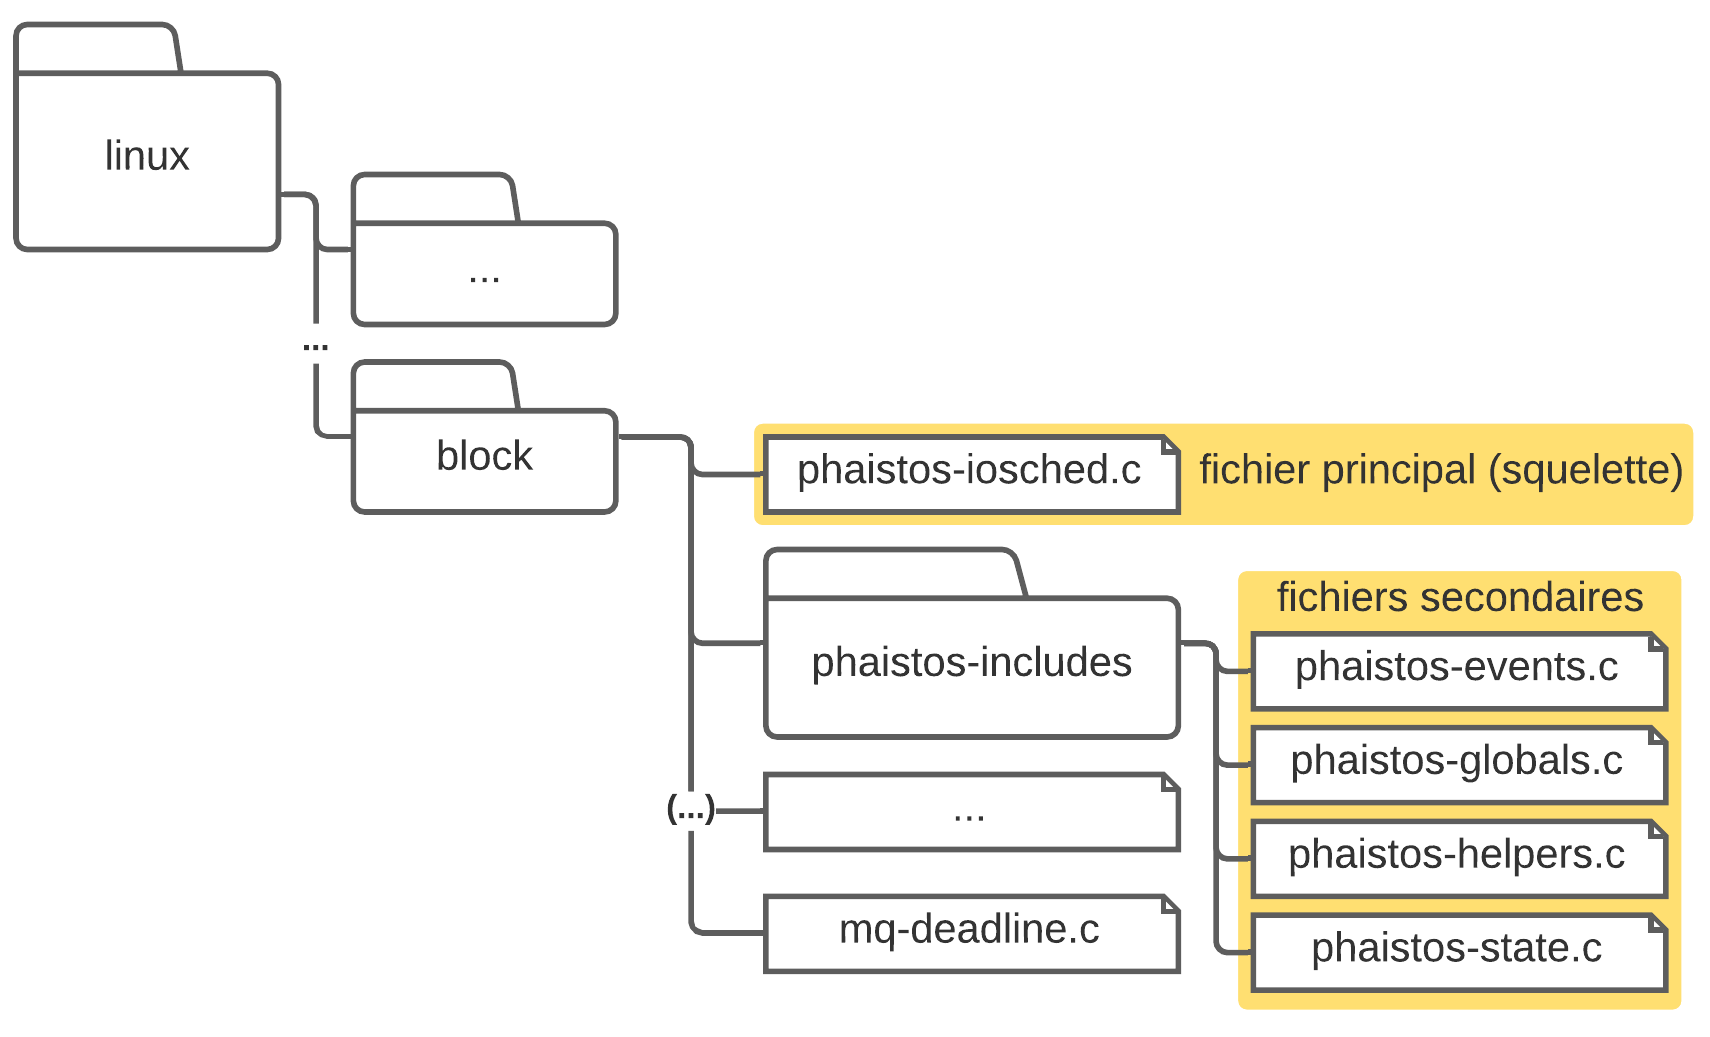
\includegraphics[width=0.8\textwidth]{images/linux_arch}
    \caption{Schéma de l'arborescence du dossier \texttt{block} dans le code 
    source Linux, augmenté par PhaistOS}
    \label{fig:modules_folder}
\end{figure}

Mon objectif était ici de changer cette méthode d'implémentation, et de faire 
en sorte que le code généré puisse être indépendant (on peut créer autant de 
politique qu'on le souhaite, sans que celles-ci se marchent dessus) et qu'il 
soit intégrable à chaud dans le noyau.

Pour cela j'ai commencé par me renseigner sur les autres ordonnanceurs, et j'ai 
appris que l'ordonnanceur Kyber, développé par Facebook, était un module que 
l'on pouvait imbriquer et désimbriquer à volonté. 

Premièrement, j'ai appris comment créer mon propre module : il me fallait 
une recette, autrement dit un Makefile, ainsi qu'un fichier \texttt{.mk} 
contenant une liste de dépendances si nécessaire. Le code généré devait avoir 
certaines particularités pour s'enregistrer auprès du système en tant que 
module, et bien heureusement PhaistOS comportait déjà ces pré-requis dans son 
fichier principal qui servait de squelette.

Deuxièmement, j'ai du modifier la génération pour qu'elle soit plus dynamique, 
cela inclu le fichier principal qui devait pouvoir s'enregistrer auprès du 
système sous différents noms, pour ne pas provoquer d'erreur à l'insertion du 
module. Comme on peut le voir dans la Figure~\ref{fig:module_name_c}, le modèle 
\texttt{script} qui sert de point d'entrée dans l'AST (comme on l'a vu dans la 
Partie~\ref{ast_files}) a été modifié pour que celui-ci génère le squelette 
ainsi que les fichiers secondaires. Dans cet extrait on retrouve les 
délimiteurs \texttt{[\$} et \texttt{\$]} qui je rappelle vont produire une 
sortie textuelle de leur contenu, autrement dit, dans ce cas il s'agit du nom 
du module choisi par l'utilisateur. Dans ce même modèle, la génération des 
fichiers secondaires est restée quasiment inchangée.

\begin{figure}[h!t] \centering
    \begin{tabular}{c}
        \begin{lstlisting}[language=Phaistos-Template, linewidth=11.5cm]
    ...
    .elevator_attrs = deadline_attrs,
    .elevator_name = \"[$!Globals.module_name$]\",
    .elevator_alias = \"[$!Globals.module_name$]\",
    .elevator_owner = THIS_MODULE,
};
MODULE_ALIAS(\"[$!Globals.module_name$]\");
...
        \end{lstlisting}
    \end{tabular}
    \caption{Extrait du modèle \texttt{script} s'occupant de la génération du 
    squelette}
    \label{fig:module_name_c}
\end{figure}

Ici, le code C qu'il y a dans le modèle de la Figure~\ref{fig:module_name_c} va 
servir à définir le contenu d'une structure qui va être donnée à une fonction 
du système qui va lire cette structure et enregistrer un nouvel ordonnanceur 
d'E/S. Cette fonctionnalité n'est pas présente pour tout les types 
d'ordonnanceurs et peut rendre la tâche beaucoup plus complexe quand elle est 
manquante. Par exemple, pour le projet Ipanema~\cite{lepers2020provable}, le 
noyau Linux est modifié pour pouvoir changer dynamiquement la politique 
d'ordonnancement des processus. Ce travail d'intégration demande beaucoup plus 
de temps et d'effort, mais heureusement, les développeurs Linux l'ont déjà fait 
dans notre cas (merci).

Troisièmement, il fallait ajouter la génération d'un fichier \texttt{.mk} qui 
allait permettre de lister les dépendances nécessaires au bon fonctionnement du 
module. Pour cela j'ai donc ajouté une règle \texttt{let! mk\_file} au modèle 
\texttt{script}, produisant directement une sortie sans parcourir l'AST.

Pour finir, il a fallu écrire le Makefile pour gérer les différentes phases de 
génération du code C propre au module (fichier principale, secondaires et 
fichier \texttt{.mk}), ainsi que son exportation vers le dossier \texttt
{Output-Modules}, dans un sous-dossier spécifique, accompagné d'un Makefile 
pour compiler le module et intégrer le nouvel ordonnanceur d'E/S au système.

\begin{center}
---
\end{center}
    
J'ai donc trouvé un moyen relativement simple de générer un code C directement 
compilable et intégrable dans le noyau Linux en tant que module. Pour cela un 
Makefile dédié à cet effet et une modification de la génération par les modèles 
sont à l'origine de ce changement. De plus, la modification d'un noyau Linux 
n'est plus nécessaire puisque la notion de module existe de base dans le 
système.

\subsection{Mise en place d'une machine virtuelle pour les tests}

Pour effectuer des tests de fonctionnement ou de compatibilité, j'avais besoin 
de travailler sur un environement de travail robuste (de bonnes performances 
pour les compilations noyau ou autre) et sûr (pas de pertes en cas de crash). 
Pour la robustesse j'ai donc utilisé les serveurs Grid'5000 et pour la sûreté 
j'ai décidé de reprendre ce qu'avait laissé Nick derrière lui, c'est à dire une 
image système enregistrée par le logiciel de virtualisation Qemu.

L'image laissée en l'état par Nick comportait le noyau Linux modifié ainsi que 
l'ordonnanceur Deadline généré par le DSL, il y avait aussi certains scripts 
présents pour changer d'ordonnanceur ou pour effectuer des tests de 
performances rapides. Le problème avec cette image c'est qu'elle ne m'a servit 
qu'au début du stage pour comprendre comment PhaistOS fonctionnait, mais 
j'avais besoin de créer ma propre image, avec mon propre environement pour 
tester la nouvelle implémentation exposée en Partie~\ref{module}.

Pour cela j'ai modifié le contenu du dossier ``Matryoshka'' (voir Figure~\ref
{fig:arch}) sur ma branche de développement Git. J'ai principalement apporté 
des modifications aux scripts de mise en place de l'image Qemu, mais j'ai aussi 
supprimé le contenu du dossier \texttt{linux} qui contenait le SE modifié (le 
dossier me servira encore pour le téléchargement du noyau qui sera compilé par 
les scripts).

Le script principal de mise en place de Qemu et d'installation du système a 
été le plus compliqué à écrire. En effet ce script va permettre d'effectuer une 
installation propre de tout un système debian de base avec un noyau Linux 
version 5.13 non modifié. Ce système sera compilé et sauvegardé dans une image 
Qemu par ce script, pour qu'il puisse être démarré ou monté à volonté. La 
difficulté d'écriture d'un tel script résidait dans la maîtrise des outils qui 
lui sont nécessaires. Le script est disponible en annexe (voir Figure~\ref
{fig:script}) mais voici un récapitulatif de ses différentes étapes :

\begin{enumerate}
    \item Installation de dépendances, définition des variables et nettoyage 
    des précédentes installations.
    \item Téléchargement et compilation d'un noyau Linux avec la bonne 
    configuration pour accueillir des modules.
    \item Mise en place d'une image Qemu :
    \begin{enumerate}
        \item Création du fichier contenant l'image.
        \item Création d'une partition au format ext4 dans l'image.
        \item Téléchargement d'un système de base d'une debian buster (version 
        10) sur cette partition.
    \end{enumerate}
    \item Montage de l'image et configuration interne du système (modifications 
    de fichiers et d'installations importantes pour que la VM fonctionne 
    correctement). Cela comprend la liaison virtuelle nécessaire pour que Qemu 
    puisse voir le code source Linux (contenu dans le dossier \texttt{linux}) 
    nécessaire pour la compilation des modules.
    \item Copies des modules actuellement générés dans l'image où ils 
    attendront d'être compilés par l'utilisateur.
\end{enumerate}

Des scripts secondaires existent et ont pour but de lancer la machine virtuelle 
avec l'image préalablement créée. Certains permettent aussi de monter l'image 
dans un dossier pour qu'elle puisse être visible comme le contenu d'un disque 
dur.

\begin{center}
---
\end{center}
    
La machine virtuelle reste une valeur de sûreté car elle permet au développeur 
d'effectuer ses expérimentations sans mettre en danger son système, ce bac à 
sable est l'endroit idéal pour développer des politiques d'ordonnancement 
personnalisées. Grâce à cette mise en oeuvre le prochain développeur qui 
travaillera sur PhaistOS pourra mettre en place une machine virtuelle 
facilement avec la configuration requise pour expérimenter ses politiques et 
faire des tests avec le DSL. Une fois son DSL stable il pourra ensuite passer à 
des choses plus sérieuses en le testant sur des machines physiques.

\subsection{Tests d'analyse de performances}

Le but dans cette partie est de montrer que l'utilisation d'un DSL n'a que très 
peu d'impacte sur les performances finales des politiques PhaistOS.

<reprendre plos21.pdf>

\begin{center}
---
\end{center}
    
<mini-résumé>
